\documentclass[a4paper, 11pt]{article}
\usepackage{amsmath}
\usepackage{graphicx}
\usepackage{geometry}
\usepackage{listings}
\usepackage[colorlinks,linkcolor=red]{hyperref}
\geometry{scale=0.8}

\title{	
\normalfont \normalsize
\textsc{School of Data and Computer Science, Sun Yat-sen University} \\ [25pt] %textsc small capital letters
\rule{\textwidth}{0.5pt} \\[0.4cm] % Thin top horizontal rule
\huge  Maze Problem\\ % The assignment title
\rule{\textwidth}{2pt} \\[0.5cm] % Thick bottom horizontal rule
\author{16110917 Zhaoshuai Liu}
\date{\normalsize\today}
}

\begin{document}
\maketitle
\tableofcontents
\newpage
\section{Task}



\begin{itemize}
	\item Please solve the maze problem (i.e., find the shortest path from the start point to the finish point) by using BFS or DFS (Python or C++)
	\item The maze layout can be modeled as an array, and you can use the data file \texttt{MazeData.txt} if necessary.
	\item Please send \texttt{E01\_YourNumber.pdf} to \texttt{ai\_201901@foxmail.com}, you can certainly use \texttt{E01\_Maze.tex} as the \LaTeX template.
\end{itemize}

\begin{figure}[ht]
\centering
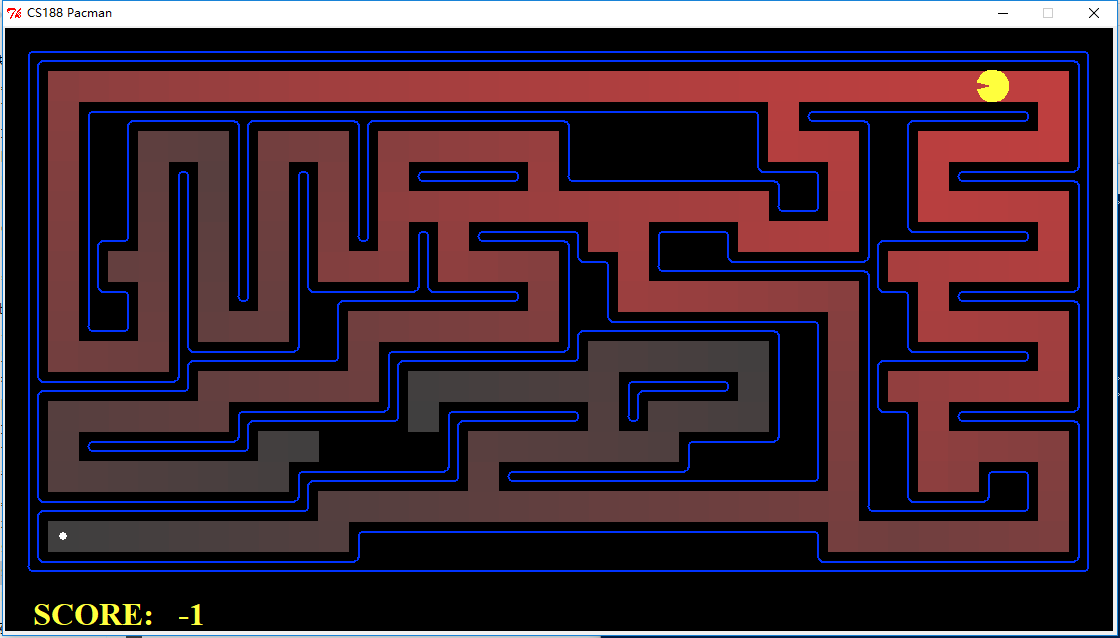
\includegraphics[width=15cm]{Pic/Pacman}

\caption{Searching by BFS or DFS}
\end{figure}
\section{Codes}
\lstset{language=C++}
%%\lstset{language=Python}
\begin{lstlisting}

\end{lstlisting}
\section{Results}
\begin{figure}
\centering
%%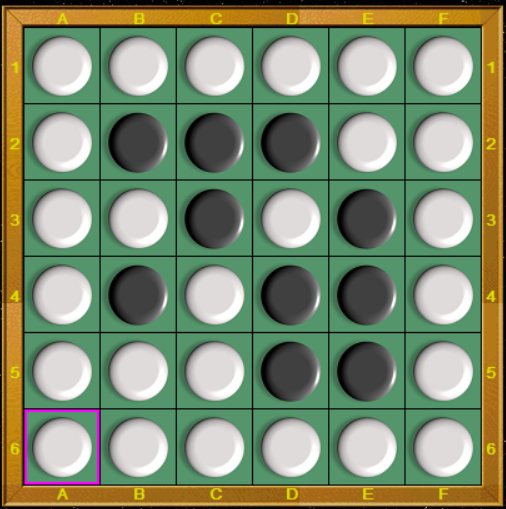
\includegraphics[width=15cm]{result.png}
\end{figure}


%\clearpage
%\bibliography{E:/Papers/LiuLab}
%\bibliographystyle{apalike}
\end{document} 